\enteteExam{NFP 107 -- Systèmes de gestion de bases de données - Durée 2h30}%
{Examen session 2 -- 22 Janvier 2025}%
{Examen sur table -- Seuls documents autorisés\,: 10 pages maximum de notes personnelles.}%

On s'intéresse au système d'information d'une station de ski. Elle propose
des remontées mécaniques pour accéder à des pistes. Une piste
peut être desservie par plusieurs remontées, et une remontée peut desservir 
plusieurs pistes.
La station propose
aux skieurs d'accéder à chaque remontée mécanique moyennant un tarif 
appliqué à chaque passage. 
Un cumul des passages par skieur est effectué
                 en fin de journée, et le montant obtenu
                est prélevé sur le compte du skieur.

Un concepteur propose le schéma suivant; les clés primaires sont en gras.

\begin{itemize}
\item Skieur(\textbf{id}, nom, prénom, noMobile)
\item Remontée (\textbf{id}, intitulé, tarif)
\item Piste(\textbf{id}, nom, couleur, longueur)
\item Passage(\textbf{id}, jour, heure, idSkieur, idRemontée)
\item AccèsPiste(\textbf{idRemontée, idPiste})

\end{itemize}

\subsection*{Conception du schéma (7 pts)}

\begin{enumerate}
 \item Aurait-on pu choisir comme clé de la table \texttt{Passage}
      la paire d'attributs (idSkieur, idRemontée)\,? Donnez vos arguments pour ou contre
      un tel changement.
       
  \item Le schéma permet-il de savoir sur quelles pistes est passé un skieur?
  
 \item Donnez les commandes SQL de création des tables \texttt{Remontée}, \texttt{Piste}
 et \texttt{AccèsPiste}.
        
   \item On veut affecter des employés de la station aux  
   remontées mécaniques pour effectuer l'entretien, le contrôle des skieurs,
     et l'assistance éventuelle. On part d'une relation \texttt{Affectation}
     avec les attributs
       \texttt{(idRemontée, intitulé, tarif, idEmployé, nom, dateEmbauche)} 
       et les dépendances fonctionnelles suivantes\,:
  \begin{itemize}
    \item \texttt{idEmp -> nom, dateEmbauche}
    \item \texttt{idRemontée -> intitulé, tarif}
  \end{itemize}

   Donnez la clé de \texttt{Affectation}. Est-celle en 3FN (justifiez)\,?
   Si non indiquez sa décomposition en 3FN par 
   application de l'algorithme de normalisation (2 pts).
   
 \item Quel est d'après vous le schéma entité-association 
        correspondant au schéma relationnel obtenu (2 pts)\,?
\end{enumerate}

   
\begin{solution}

\begin{enumerate}
   \item Un skieur peut sans aucun doute accéder plusieurs fois à la même
     remontée. Choisir la paire comme clé n'est donc pas du tout une bonne idée.
    \item On sait quelles remontées a pris un skieur, mais ça ne dit
    pas quelle piste a été choisie ensuite. Donc, non. 
  
    \item  On note que les clés étrangères sont \textit{idSkieur} et \textit{idRemontée} dans
  la table \texttt{Passage}\,;  \textit{idPiste} et \textit{idRemontée}
  dans la table \texttt{AccèsPiste}. Voici le schéma pour \texttt{AccèsPiste}\,:
    
\begin{minted}{sql}
   create table AccèsPiste  (idRemontée integer not null, 
                        idPiste    integer not null, 
                        primary key (idRemontée, idPiste),
                        foreign key (idRemontée) references Remontée(id),
                        foreign key (idPiste) references Piste(id));
  \end{minted}
    
  \item La clé est \texttt{(idRemontée, idEmployé)}, ce qui indique 
     qu'un employé peut être affecté à plusieurs remontées.  \texttt{Affectation}
     n'est pas en 3FN car, pour les deux DF données, la partie gauche n'est pas la clé.
     Après normalisation, on retrouve la table \texttt{Remontée},
     une nouvelle table \texttt{Employé} et une table \texttt{Affectation}
     avec pour clé \texttt{idRemontée, idEmployé}.
     
  \item La figure~\ref{station} montre le schéma E/A, avec les employés. NB\,:
dans une étape ultérieure, il sera préférable  de créer une seule entité regroupant les skieurs
et les employés (qui ont le droit sans doute de skier
pendant leur période de congé). 

  \begin{figure}[htb]  
   \centerline{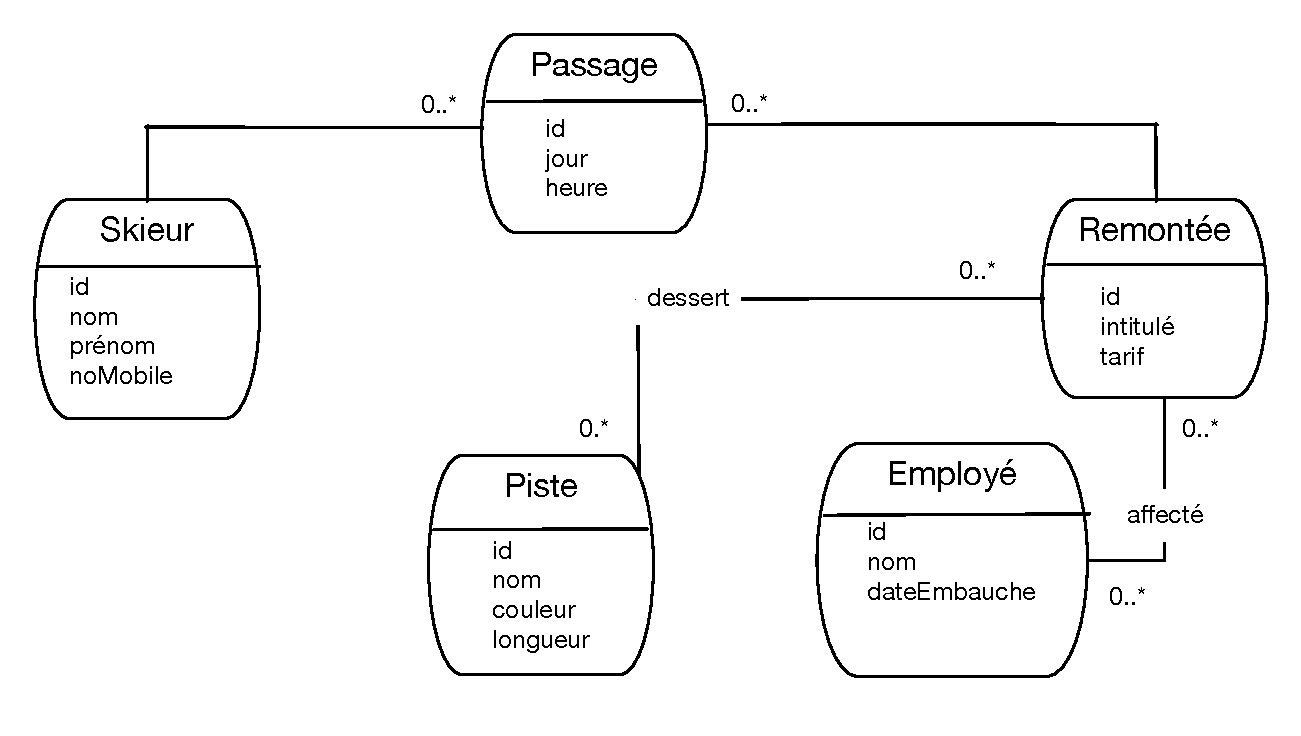
\includegraphics[scale=0.5]{../supports/figures/exam-20-stationski}}
    \caption{Modèle de la station de ski}  
    \label{station}  
  \end{figure}  
\end{enumerate}  
  
\end{solution}

\subsection*{SQL (6 pts)}

Sur le schéma obtenu précédemment, exprimez en SQL les requêtes suivantes\,:

\begin{enumerate}
   \item Intitulé des remontées donnant accès aux pistes dont la longueur est 
         supérieure à 1\,500 m. 

  \item Donnez l'id des remontées empruntées par le skieur Gilles Carpet
  sous trois formes équivalentes\,: 
     déclarative, algébrique et avec imbrication (2 pts)
 
  \item Quelle requête SQL permet d'afficher un tableau à deux colonnes
     avec le nom d'une piste en colonne 1 et le nom d'une remontée
     desservant la piste en colonne 2. Important\,: si une piste
     n'est desservie par aucune remontée on veut qu'elle apparaisse quand 
     même une fois.  
      
   \item Quels skieurs (prénom, nom) n'ont jamais pris la remontée intitulée "Marmottes"\,?

   \item À combien de pistes donne accès la remontée  \guill{Génépi}\,?

 
\end{enumerate}


\begin{solution}

\begin{enumerate}

\item 
\begin{minted}{sql}
select intitulé 
from  Remontée as r, Piste as p, AccèsPiste as a 
where r.id = a.idRemontée 
and   p.id = a .idPiste 
and p.longueur > 1500
\end{minted}


\item Déclaratif\,:

\begin{minted}{sql}
select idRemontée 
from  Passage as p, Skieur as s
where s.prénom='Gilles' and s.nom='Carpet'
and p.idSkieur = s.id
\end{minted}

Algébrique\,:

\begin{minted}{sql}
select idRemontée 
from  Passage as p join Skieur as s on p.idSkieur = s.id
where s.prénom='Gilles' and s.nom='Carpet'
\end{minted}


Imbrication\,:

\begin{minted}{sql}
select idRemontée 
from  Passage as p 
where p.idSkieur in (select s.id
                     from Skieur
                     where s.prénom='Gilles' and s.nom='Carpet')
\end{minted}

\item  Il faut une jointure externe pour être assuré d'afficher les pistes sans accès.
   Si c'est le cas, \texttt{r.intitulé} sera à \texttt{null}.
\begin{minted}{sql}
select p.nom, r.intitulé
from   Piste as p outer join 
           (AccèsPiste as a join Remontée as r 
               on a.idRemontée = r.id) 
        on p.id = a .idPiste 
\end{minted}


\item 
\begin{minted}{sql}
select prénom, nom
from  Skieur as s
where not exist (select *
              from Remontée as r, Passage as p
               where p.idSkieur=s.id
               and p.idRemontée = r.id
               and r.intitulé = 'Marmottes' )
\end{minted}


\item 
\begin{minted}{sql}
select count(*)
from  Remontée as r, as r, Piste as p, AccèsPiste as a 
where r.id = a.idRemontée 
and   p.id = a .idPiste 
and r.intitulé = 'Génépi'
\end{minted}



\end{enumerate}

\end{solution}



\subsection*{Algèbre (2 pts)}

Donnez l'expression algébrique correspondant 
à la requête 4 (skieurs qui 
n'ont jamais pris la remontée intitulée "Marmottes").


\subsection*{Vues (3 pts)}

\begin{enumerate}
   \item Créez une vue \texttt{Fréquentation} donnant,  pour chaque skieur
        et chaque jour de son séjour, son nom, 
       le nombre de remontées empruntées et le cumul des tarifs.
     
      \item En utilisant cette vue, quelle requête donne les skieurs
        qui ont emprunté plus de 20 remontées (afficher 
        le nom du skieur et le jour).
\end{enumerate}

\begin{solution}

\begin{minted}{sql}
create view Fréquentation as
select  s.nom, p.jour, count(*) as 'nbRemontées', sum(tarif) as 'cumulTarif'
from  Skieur as s, Remontée as r, Passage as p
where  p.idRemontée = r.id
and s.id = p.idSkieur
group by s.id, p.jour
\end{minted}

On peut interroger cette vue très simplement\,:
\begin{minted}{sql}
select nom, jour
from Fréquentation
where  nbRemontées > 20
\end{minted}

\end{solution}

\subsection*{Transactions (2 pts)}

Les propriétés d'une transaction sont résumées 
par l'acronyme ACID. Rappeler brièvement le sens de
ces quatre propriétés.


\begin{solution}
Voir cours
\end{solution}
\end{document}


\subsection*{Indexation (3 pts)}

\`A la fin de la saison, 250\,000 skieurs
ont fréquenté la station. On stocke
les données dans une base ORACLE avec des blocs
de 4\,000 octets, et on 
suppose que chaque ligne de la table \texttt{Skieur} occupe
200 octets sur le disque. 
 Répondez aux questions suivantes en justifiant
    vos réponses (on suppose que les pages sont pleines
   et on ne tient pas compte de la mémoire cache).
  \begin{enumerate}
   \item Quelle est la taille du segment de données pour 
           la table \texttt{Skieur} (en blocs, et en octets)\,? 


  \item L'identifiant du skieur est un entier sur 4 octets,
         et l'adresse d'un bloc occupe 16 octets. Décrivez
          la structure de l'arbre B+ sur l'id, et donnez son nombre de niveaux
         en fonction des chiffres précédents. 

  \item En supposant qu'il faut 10ms pour lire un bloc, 
         quel est le temps {\em moyen} de recherche d'un skieur
         par son identifiant GPS en supposant qu'il n'y a pas d'index\,?
       Quel est le temps d'accès à un skieur en fonction de son id\,?

\begin{solution}
\begin{enumerate}
  \item 50 Mo!
  \item $\frac{50000000}{4000}=12500$
\end{enumerate}
\end{solution}
\begin{solution}
   \item Quelle est la taille d'un index de type arbre-B
        si la clé fait 32 octets
           et un pointeur 8 octets\,?

Une entrée d'index fait 40 octets. Donc on en met
$\frac{4000}{40}=100$ par page. Il faut indexer 1\,000\,000
enregistrements pour le dernier niveau de l'index, soit
$\frac{1000000}{100}=10000$ pages. Ensuite il
faut indexer chacune des 1000 pages, soit $\frac{1000}{100}=10$
pages supplémentaires, que pour finir on indexe avec la racine.

Donc il faut 10000 + 10 + 1 pages dans l'index.
\end{solution}
 \begin{solution}
 
   \item  Si on suppose qu'un E/S coûte 10 ms, quel est le coût moyen
    d'une recherche
     d'un enregistrement par clé unique,
   avec index et sans index\,?


Recherche avec index\,: trois lectures dans l'index, 
puis une lecture dans le fichier. Soit 40 ms.

Sans index, en moyenne il faut lire la moitié du fichier,
soit 5625 pages, soit plus de 50 secondes.
\end{solution}
\end{enumerate}


\subsection*{\'Evaluation de requêtes (3 pts)}

On veut donner le nom de toutes les remontées
mécaniques qui sont de type \guill{Téléski}. Bien entendu, on suppose
que la table stockant les types est considérablement plus petite
que la table stockant les remontées.

\begin{enumerate}
   \item Donner la requête SQL.
   \item Donner l'expression algébrique correspondante.
    \item Donner au moins deux plans d'exécution possibles, sous la 
             forme qui vous convient.
          Quel est le meilleur d'après vous\,? Quels
     index peut-on créer pour améliorer les performances de cette requête\,?

\end{enumerate}
